\documentclass[../../../../main.tex]{subfiles}
\begin{document}

\section{Main Border Pane}
When I created a \texttt{JavaFX} project in the Eclipse IDE, it automatically created a main pane and a template for initializing the scene and loading the pane. I added a few lines of code to control how big the window will originally be.
\begin{minted}[
frame=lines,
framesep=2mm,
linenos,
breaklines
]{java}
package application;

import javafx.application.Application;
import javafx.stage.Stage;
import javafx.scene.Scene;
import javafx.scene.layout.BorderPane;
import javafx.fxml.FXMLLoader;

public class Main extends Application {
	
	// methods
	@Override
	// a method to start the gui
	public void start(Stage primaryStage) {
		try {
			// load the main FXML file
			BorderPane root = (BorderPane) FXMLLoader.load(getClass().getResource("Main.fxml"));
			// create the scene with the borderpane as the root node
			Scene scene = new Scene(root);
			scene.getStylesheets().add(getClass()
				.getResource("application.css").toExternalForm());
			primaryStage.setScene(scene);
			// make the window 1020 x 720 big
			primaryStage.setHeight(720);
			primaryStage.setWidth(1020);
			// show the window
			primaryStage.show();
		} catch (Exception e) {
			e.printStackTrace();
		}
	}
	
	// run the program
	public static void main(String[] args) {
		// launch the gui
		launch(args);
	}
}
\end{minted}
After I edited this main class, I opened the main \texttt{BorderPane FXML} file in scene builder. I removed all the automatically generated regions and gave the main pane a \texttt{fxid} which basically allows, me to access it in the controller class.

\begin{figure}[H]
	\begin{center}
		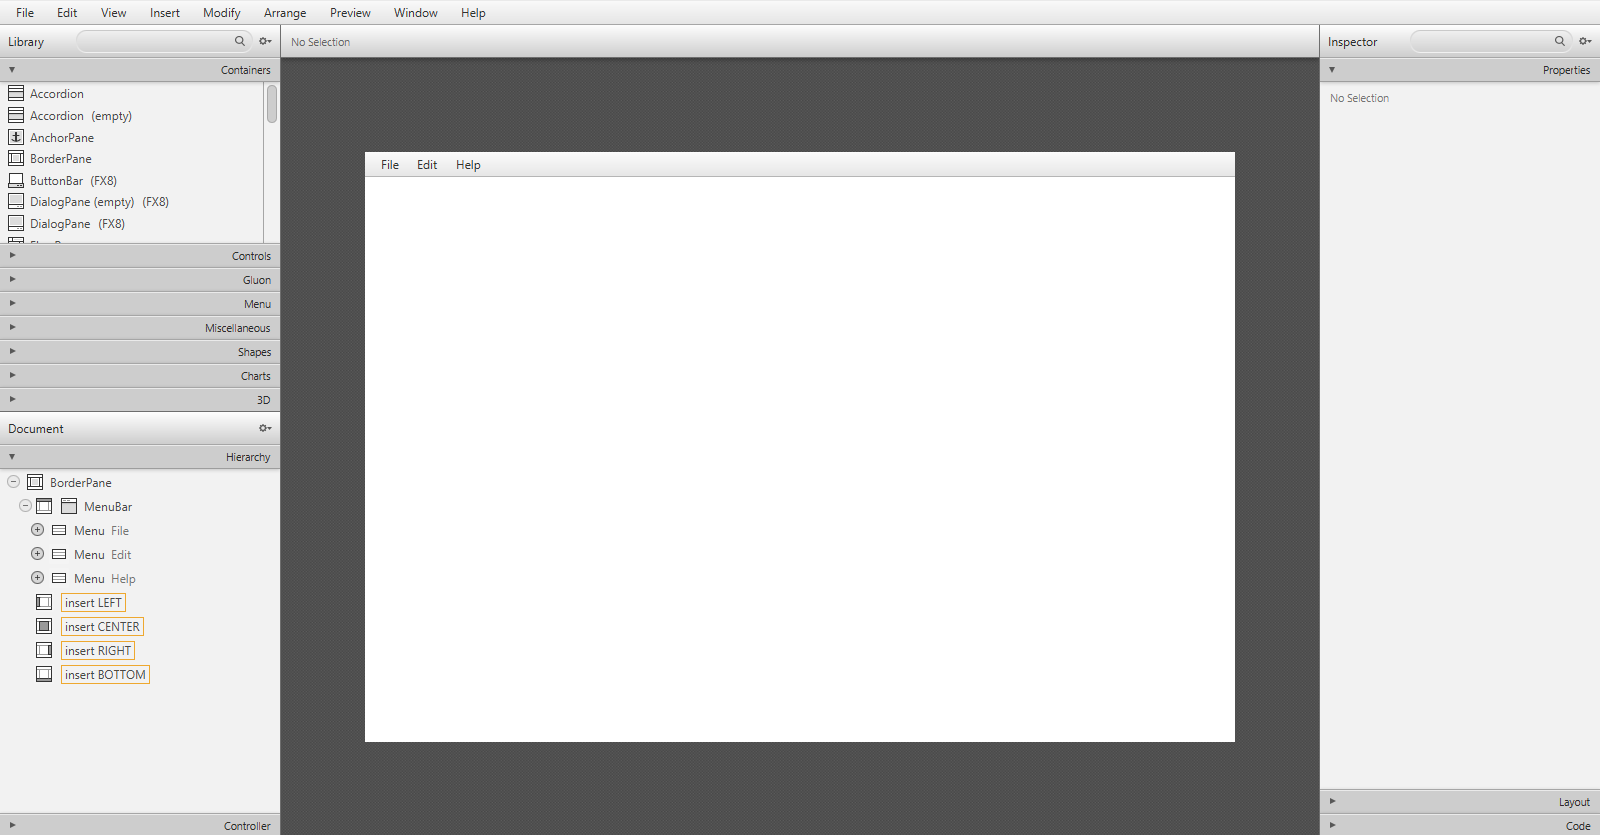
\includegraphics[width=0.9\textwidth]{images/mainFXML}
	\end{center}
	\caption{Creating the Main Pane in Scene Builder}
\end{figure}

The \texttt{FXML} for this pane is shown below:

\begin{minted}[
frame=lines,
framesep=2mm,
linenos,
breaklines,
fontsize = \fontsize{9}{9}
]{xml}
<?xml version="1.0" encoding="UTF-8"?>

<?import javafx.scene.control.Menu?>
<?import javafx.scene.control.MenuBar?>
<?import javafx.scene.control.MenuItem?>
<?import javafx.scene.layout.BorderPane?>

<BorderPane fx:id="rootPane" prefHeight="590.0"
	prefWidth="870.0" xmlns="http://javafx.com/javafx/8.0.141"
	xmlns:fx="http://javafx.com/fxml/1"
	fx:controller="application.MainController">
	<top>
		<MenuBar BorderPane.alignment="CENTER">
			<menus>
				<Menu mnemonicParsing="false" text="File">
					<items>
						<MenuItem mnemonicParsing="false" text="Close" />
					</items>
				</Menu>
				<Menu mnemonicParsing="false" text="Edit">
					<items>
						<MenuItem mnemonicParsing="false" text="Delete" />
					</items>
				</Menu>
				<Menu mnemonicParsing="false" text="Help">
					<items>
						<MenuItem mnemonicParsing="false" text="About" />
					</items>
				</Menu>
			</menus>
		</MenuBar>
	</top>
</BorderPane>
\end{minted}
\newpage \noindent
I then created a corresponding controller file in which I initialized a \texttt{PlotPane} and set it as the center node in the border pane:
\begin{minted}[
frame=lines,
framesep=2mm,
linenos,
breaklines
]{java}
package application;

import javafx.fxml.FXML;
import javafx.fxml.Initializable;
import javafx.scene.layout.BorderPane;

public class MainController implements Initializable {

	@FXML
	private BorderPane rootPane;

	@Override
	public void initialize(URL arg0, ResourceBundle arg1) {
		// initialize the plotpane
		PlotPane plotPane = new PlotPane();
		// add the panes to the root pane
		rootPane.setCenter(plotPane);
	}

}
\end{minted}
I then tested if the program would run without crashing, expecting to see a pair of axes:
\begin{figure}[H]
	\begin{center}
		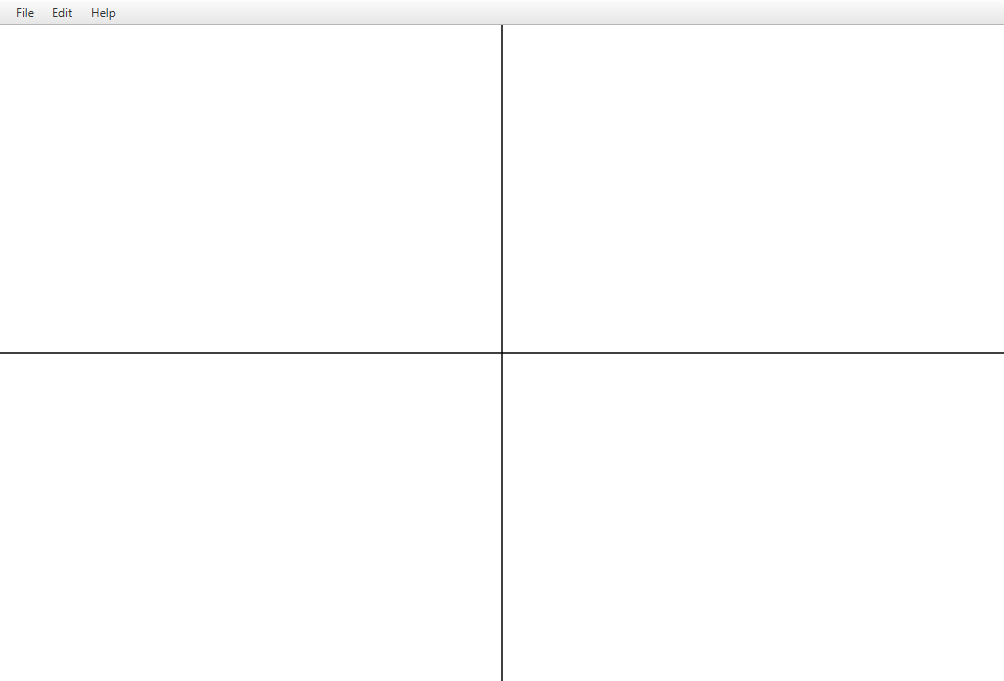
\includegraphics[width=0.7\textwidth]{images/test}
	\end{center}
	\caption{Creating the Main Pane in Scene Builder}
\end{figure}
And I saw exactly that.
\newpage
\end{document}